\documentclass[12pt,aspectratio=169]{beamer}
\usepackage[utf8]{inputenc}
\usepackage[T1]{fontenc}
\usepackage{graphicx}
\usepackage{tikz}
\usetikzlibrary{positioning, shapes.geometric, arrows.meta, calc}
\usepackage{amsmath}
\usepackage{amssymb}
\usepackage{xcolor}
\usepackage{hyperref}
\usepackage{tikz}
\usetikzlibrary{positioning, arrows.meta} % <-- important for right=of, below=of and arrows

\usepackage{tikz}
\usetikzlibrary{positioning, arrows.meta} % <-- required for right=of and arrows
\usetikzlibrary{positioning}




% Modern theme
\usetheme{Madrid}
\usecolortheme{seahorse}

% Custom colors
\definecolor{myblue}{RGB}{0,102,204}
\definecolor{myorange}{RGB}{255,128,0}
\definecolor{mygreen}{RGB}{34,139,34}
\definecolor{mypurple}{RGB}{128,0,128}

\setbeamercolor{structure}{fg=myblue}
\setbeamercolor{frametitle}{bg=myblue,fg=white}

% Document information
\title[Introduction to ML]{Introduction to Machine Learning}
\subtitle{Automated Learning}
\author{Meyssem Bouzaien}
\date{Academic Year: 2025 - 2026}

\begin{document}

% Title page
\begin{frame}
\titlepage
\end{frame}

% Outline
\begin{frame}{Outline}
\tableofcontents
\end{frame}

% ============================================
% SECTION 1: WHAT IS ML
% ============================================
\section{What is Machine Learning?}

\begin{frame}{Reminder: AI vs Machine Learning}
\begin{center}
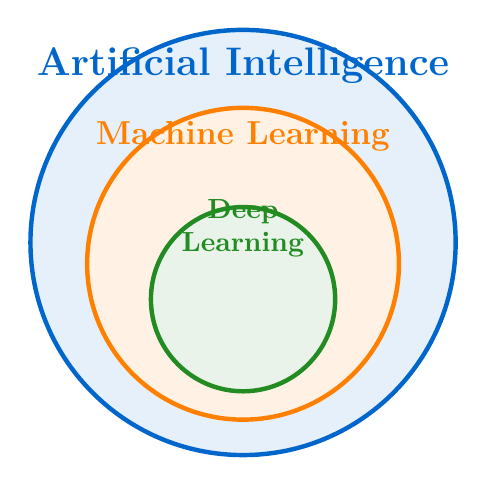
\begin{tikzpicture}[scale=0.9]
% AI circle
\draw[ultra thick, myblue, fill=myblue!10] (0,0) circle (3cm);
\node[myblue] at (0,2.5) {\Large \textbf{Artificial Intelligence}};

% ML circle
\draw[ultra thick, myorange, fill=myorange!10] (0,-0.3) circle (2.2cm);
\node[myorange] at (0,1.5) {\large \textbf{Machine Learning}};

% DL circle
\draw[ultra thick, mygreen, fill=mygreen!10] (0,-0.8) circle (1.3cm);
\node[mygreen, text width=2cm, align=center] at (0,0.2) {\textbf{Deep Learning}};
\end{tikzpicture}
\end{center}

\textbf{Where ML Fits}
Machine Learning is the branch of AI that enables machines to learn from data
\end{frame}

\begin{frame}{What is Machine Learning?}
\begin{definition}[Machine Learning]
Machine Learning is the study of computer algorithms that improve automatically through experience and the use of data.
\end{definition}


\begin{columns}[T]
\column{0.5\textwidth}
\textbf{Traditional Approach}
\begin{itemize}
\item Programmer writes the rules
\item Explicit logic
\item Difficult for complex tasks
\item Example: if-then-else
\end{itemize}

\column{0.5\textwidth}
\textbf{Machine Learning Approach}
\begin{itemize}
\item Machine learns the rules
\item Learning from data
\item Suited to complex tasks
\item Example: image recognition
\end{itemize}
\end{columns}
\end{frame}

\begin{frame}{Classical Programming vs Machine Learning}
\begin{center}
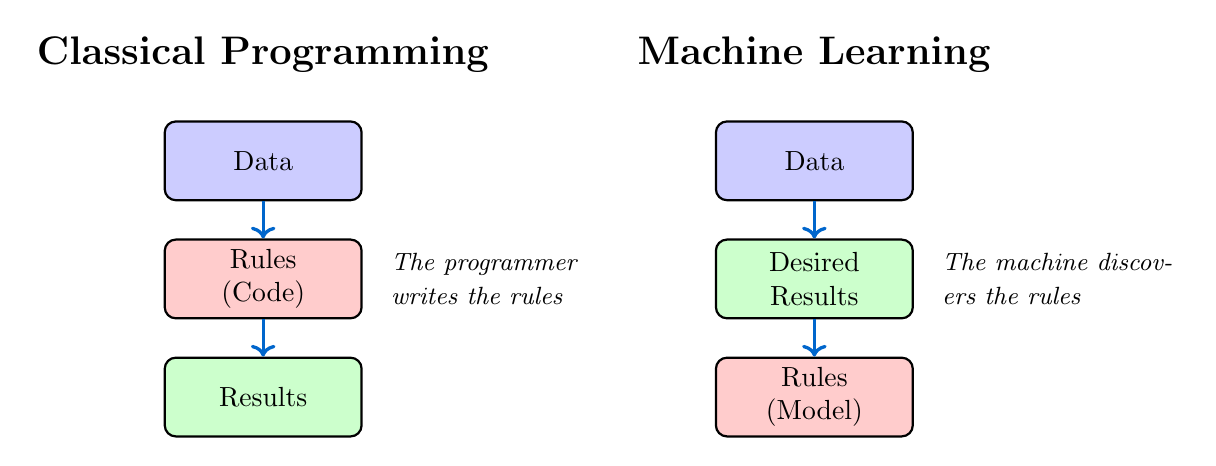
\begin{tikzpicture}[
box/.style={rectangle, draw, thick, minimum width=2.5cm, minimum height=1cm, align=center, rounded corners},
arrow/.style={->, very thick, myblue}
]

% Classical Programming
\node[above] at (0,3.5) {\Large \textbf{Classical Programming}};
\node[box, fill=blue!20] (data1) at (0,2.5) {Data};
\node[box, fill=red!20] (rules1) at (0,1) {Rules\\(Code)};
\node[box, fill=green!20] (output1) at (0,-0.5) {Results};

\draw[arrow] (data1) -- (rules1);
\draw[arrow] (rules1) -- (output1);

\node[right, text width=3cm] at (1.5,1) {\small \textit{The programmer writes the rules}};

% Machine Learning
\node[above] at (7,3.5) {\Large \textbf{Machine Learning}};
\node[box, fill=blue!20] (data2) at (7,2.5) {Data};
\node[box, fill=green!20] (output2) at (7,1) {Desired\\Results};
\node[box, fill=red!20] (rules2) at (7,-0.5) {Rules\\(Model)};

\draw[arrow] (data2) -- (output2);
\draw[arrow] (output2) -- (rules2);

\node[right, text width=3cm] at (8.5,1) {\small \textit{The machine discovers the rules}};

\end{tikzpicture}
\end{center}
\end{frame}

\begin{frame}{Why Machine Learning?}
\begin{block}{Problems That Are Hard to Program}
Some tasks are too complex to be programmed with explicit rules
\end{block}

\vspace{0.3cm}

\begin{columns}[T]
\column{0.5\textwidth}
\textbf{Examples of ML Tasks}
\begin{itemize}
\item Facial recognition
\item Spam filtering
\item Machine translation
\item Price prediction
\item Product recommendation
\item Medical diagnosis
\end{itemize}

\column{0.5\textwidth}
\textbf{Why Is It Difficult?}
\begin{itemize}
\item Too many variables
\item Complex patterns
\item Non-obvious rules
\item Data that evolves over time
\item Numerous edge cases
\item Context matters
\end{itemize}
\end{columns}
\end{frame}

% ============================================
% SECTION 2: THE ML PROCESS
% ============================================
\section{The Machine Learning Process}

\begin{frame}{The Machine Learning Pipeline}
\begin{center}
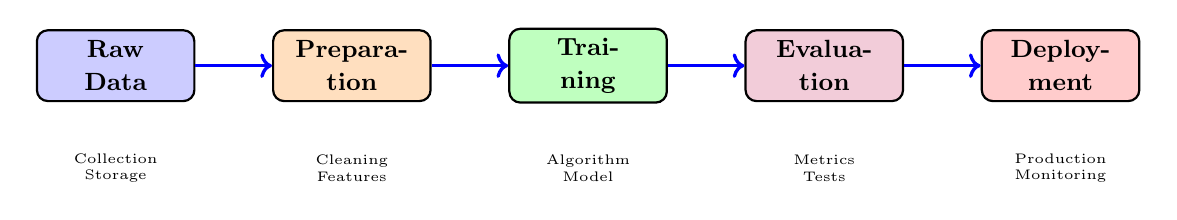
\begin{tikzpicture}
% Pipeline stages
\node[rectangle, draw=black, thick, fill=blue!20, rounded corners, 
      minimum width=2cm, minimum height=0.9cm, align=center] (data) at (0,0) 
      {\small\textbf{Raw}\\\small\textbf{Data}};

\node[rectangle, draw=black, thick, fill=orange!25, rounded corners, 
      minimum width=2cm, minimum height=0.9cm, align=center] (prep) at (3,0) 
      {\small\textbf{Prepara-}\\\small\textbf{tion}};

\node[rectangle, draw=black, thick, fill=green!25, rounded corners, 
      minimum width=2cm, minimum height=0.9cm, align=center] (train) at (6,0) 
      {\small\textbf{Trai-}\\\small\textbf{ning}};

\node[rectangle, draw=black, thick, fill=purple!20, rounded corners, 
      minimum width=2cm, minimum height=0.9cm, align=center] (eval) at (9,0) 
      {\small\textbf{Evalua-}\\\small\textbf{tion}};

\node[rectangle, draw=black, thick, fill=red!20, rounded corners, 
      minimum width=2cm, minimum height=0.9cm, align=center] (deploy) at (12,0) 
      {\small\textbf{Deploy-}\\\small\textbf{ment}};

% Arrows
\draw[->, very thick, blue] (data) -- (prep);
\draw[->, very thick, blue] (prep) -- (train);
\draw[->, very thick, blue] (train) -- (eval);
\draw[->, very thick, blue] (eval) -- (deploy);

% Annotations
\node[text width=2cm, align=center, font=\tiny] at (0,-1.3) {Collection\\Storage};
\node[text width=2cm, align=center, font=\tiny] at (3,-1.3) {Cleaning\\Features};
\node[text width=2cm, align=center, font=\tiny] at (6,-1.3) {Algorithm\\Model};
\node[text width=2cm, align=center, font=\tiny] at (9,-1.3) {Metrics\\Tests};
\node[text width=2cm, align=center, font=\tiny] at (12,-1.3) {Production\\Monitoring};

\end{tikzpicture}
\end{center}

\vspace{0.5cm}

\begin{alertblock}{An Iterative Process}
ML is a cycle: we often go back to previous steps to improve the model
\end{alertblock}
\end{frame}

\begin{frame}{Step 1: Data - The Fuel of ML}
\vspace{-0.3cm}

% Principle block
\begin{block}{Fundamental Principle}
\textbf{No data = No Machine Learning}
\end{block}

\vspace{0.3cm}

\begin{columns}[T]

\column{0.48\textwidth}
\textbf{Data types:} Structured (tables), Unstructured (text, images), Time series, Mixed\\[0.2cm]
\textbf{Data sources:} Databases, Files (CSV, JSON), APIs, Web scraping, IoT sensors

\column{0.48\textwidth}
\textbf{Data quality:} Completeness, Accuracy, Consistency, Relevance

\vspace{0.3cm}
% Golden rule block
\setbeamercolor{block alerted title}{bg=green!50,fg=black}
\setbeamercolor{block alerted body}{bg=green!20,fg=black}
\begin{alertblock}{Golden Rule}
\textit{Garbage In, Garbage Out} — Poor-quality data → Poor-quality model
\end{alertblock}

\end{columns}
\end{frame}




\begin{frame}{Step 2: Data Preparation (1/2)}
\begin{block}{Data Cleaning}
A crucial step that can take up 60-80\% of an ML project's time!
\end{block}

\textbf{Main operations:}

\begin{enumerate}
\item \textbf{Handling missing values}
\begin{itemize}
\item Dropping rows
\item Imputation (mean, median, mode)
\item Predicting missing values
\end{itemize}

\item \textbf{Handling outliers}
\begin{itemize}
\item Statistical detection
\item Removal or correction
\end{itemize}

\item \textbf{Handling duplicates}
\begin{itemize}
\item Identification
\item Removal
\end{itemize}
\end{enumerate}
\end{frame}

\begin{frame}{Step 2: Data Preparation (2/2)}
\textbf{Transformations:}

\begin{enumerate}
\setcounter{enumi}{3}
\item \textbf{Normalization / Standardization}
\begin{itemize}
\item Bringing variables to the same scale
\item Example: rescaling all values between 0 and 1
\end{itemize}

\item \textbf{Encoding categorical variables}
\begin{itemize}
\item Turning text into numbers
\item Example: Male → 0, Female → 1
\end{itemize}

\item \textbf{Feature Engineering}
\begin{itemize}
\item Creating new variables
\item Combining existing variables
\item Example: Age computed from Date of Birth
\end{itemize}
\end{enumerate}

\begin{alertblock}{Important}
The quality of the preparation determines the quality of the final model
\end{alertblock}
\end{frame}

\begin{frame}{ML Vocabulary: Features and Labels}
\begin{center}
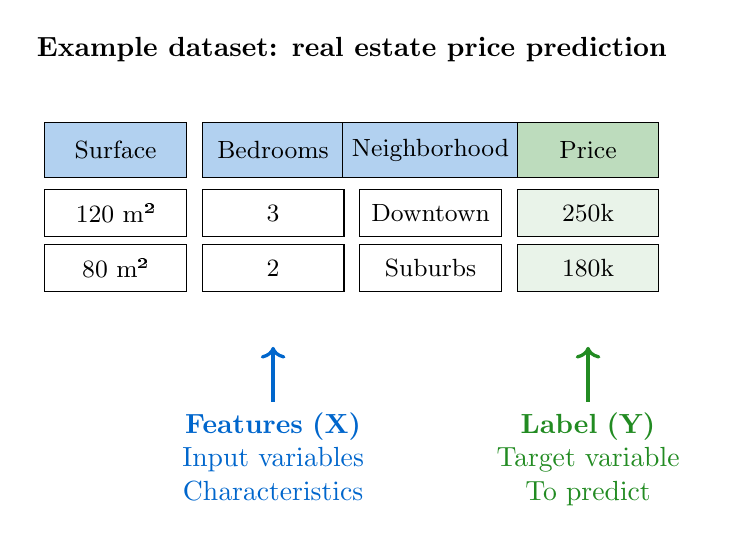
\begin{tikzpicture}
% Data table
\node[above] at (3,3) {\textbf{Example dataset: real estate price prediction}};

% Headers
\node[rectangle, draw, fill=myblue!30, minimum width=1.8cm, minimum height=0.7cm] at (0,2) {\small Surface};
\node[rectangle, draw, fill=myblue!30, minimum width=1.8cm, minimum height=0.7cm] at (2,2) {\small Bedrooms};
\node[rectangle, draw, fill=myblue!30, minimum width=1.8cm, minimum height=0.7cm] at (4,2) {\small Neighborhood};
\node[rectangle, draw, fill=mygreen!30, minimum width=1.8cm, minimum height=0.7cm] at (6,2) {\small Price};

% Row 1
\node[rectangle, draw, minimum width=1.8cm, minimum height=0.6cm] at (0,1.2) {\small 120 m²};
\node[rectangle, draw, minimum width=1.8cm, minimum height=0.6cm] at (2,1.2) {\small 3};
\node[rectangle, draw, minimum width=1.8cm, minimum height=0.6cm] at (4,1.2) {\small Downtown};
\node[rectangle, draw, fill=mygreen!10, minimum width=1.8cm, minimum height=0.6cm] at (6,1.2) {\small 250k};

% Row 2
\node[rectangle, draw, minimum width=1.8cm, minimum height=0.6cm] at (0,0.5) {\small 80 m²};
\node[rectangle, draw, minimum width=1.8cm, minimum height=0.6cm] at (2,0.5) {\small 2};
\node[rectangle, draw, minimum width=1.8cm, minimum height=0.6cm] at (4,0.5) {\small Suburbs};
\node[rectangle, draw, fill=mygreen!10, minimum width=1.8cm, minimum height=0.6cm] at (6,0.5) {\small 180k};

% Annotations
\draw[<-, very thick, myblue] (2,-0.5) -- (2,-1.2) node[below, text width=4cm, align=center] {\textbf{Features (X)}\\Input variables\\Characteristics};

\draw[<-, very thick, mygreen] (6,-0.5) -- (6,-1.2) node[below, text width=3cm, align=center] {\textbf{Label (Y)}\\Target variable\\To predict};

\end{tikzpicture}
\end{center}
\end{frame}

\begin{frame}{Step 3: Splitting the Data}
\vspace{-0.2cm}
\begin{block}{Principle}
We split the data into 2 or 3 sets to train and test the model
\end{block}

\begin{center}
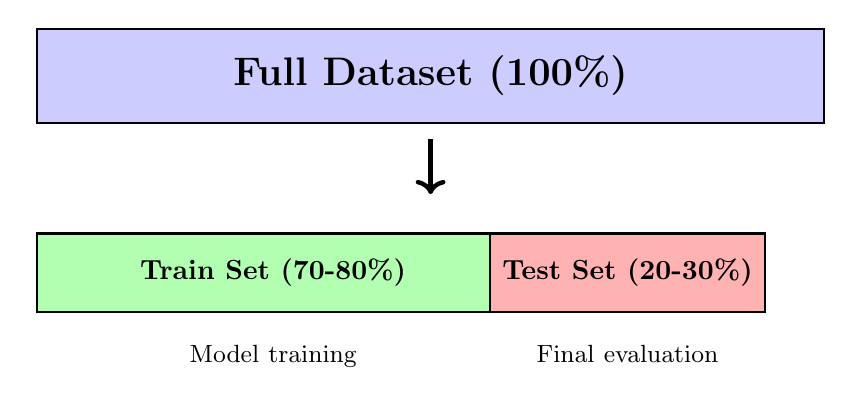
\begin{tikzpicture}
% Full dataset
\node[rectangle, draw=black, thick, fill=blue!20, minimum width=10cm, minimum height=1.2cm] (full) at (5,3) {};
\node at (5,3) {\Large \textbf{Full Dataset (100\%)}};

% Split
\draw[->, ultra thick] (5,2.2) -- (5,1.5);

% Train set
\node[rectangle, draw=black, thick, fill=green!30, minimum width=6cm, minimum height=1cm] (train) at (3,0.5) {};
\node at (3,0.5) {\textbf{Train Set (70-80\%)}};

% Test set
\node[rectangle, draw=black, thick, fill=red!30, minimum width=3.5cm, minimum height=1cm] (test) at (7.5,0.5) {};
\node at (7.5,0.5) {\textbf{Test Set (20-30\%)}};

% Annotations
\node[below, text width=6cm, align=center] at (3,-0.3) {\small Model training};
\node[below, text width=3.5cm, align=center] at (7.5,-0.3) {\small Final evaluation};

\end{tikzpicture}
\end{center}
\vspace{-0.3cm}
\begin{alertblock}{Important}
The model must NEVER see the test data during training!
\end{alertblock}
\end{frame}

\begin{frame}{Step 4: Choosing and Training the Model}
\begin{columns}[T]
\column{0.5\textwidth}
\textbf{Choosing the algorithm}
\begin{itemize}
\item Type of problem (classification, regression)
\item Nature of the data
\item Size of the dataset
\item Need for interpretability
\item Available resources
\end{itemize}

\vspace{0.3cm}

\textbf{Training}
\begin{itemize}
\item Feed the model with the training set
\item The model adjusts its parameters
\item Iterative optimization
\end{itemize}

\column{0.5\textwidth}
\begin{center}
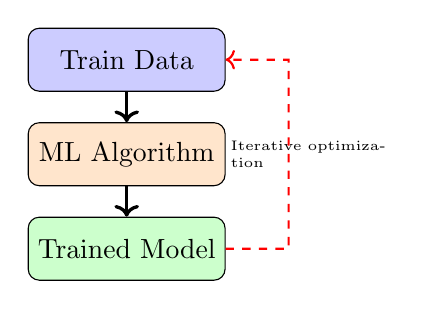
\begin{tikzpicture}[scale=0.8]
% Training process
\node[rectangle, draw, fill=blue!20, rounded corners, minimum width=2.5cm, minimum height=0.8cm] (data) at (0,3) {Train Data};

\node[rectangle, draw, fill=orange!20, rounded corners, minimum width=2.5cm, minimum height=0.8cm] (algo) at (0,1.5) {ML Algorithm};

\node[rectangle, draw, fill=green!20, rounded corners, minimum width=2.5cm, minimum height=0.8cm] (model) at (0,0) {Trained Model};

\draw[->, very thick] (data) -- (algo);
\draw[->, very thick] (algo) -- (model);

% Optimization cycle
\draw[->, thick, red, dashed] (model.east) -- ++(1,0) -- ++(0,3) -- (data.east);
\node[right, text width=2cm, font=\tiny] at (1.5,1.5) {Iterative optimization};

\end{tikzpicture}
\end{center}

\begin{block}{Result}
A model capable of making predictions on new data
\end{block}
\end{columns}
\end{frame}

\begin{frame}{Step 5: Model Evaluation}
\begin{block}{Central Question}
How do we know if our model is good?
\end{block}


\begin{center}
    \includegraphics[width=0.6\textwidth]{image.png}
\end{center}

\begin{block}{Metrics by Problem Type}
\begin{itemize}
\item \textbf{Classification}: Accuracy, Precision, Recall, F1-Score
\item \textbf{Regression}: MSE, RMSE, MAE, R²
\end{itemize}
\end{block}
\end{frame}


% ============================================
% SECTION 3: TYPES OF LEARNING
% ============================================
\section{Types of Learning}

\begin{frame}{The 3 Major Types of Learning}
\begin{center}
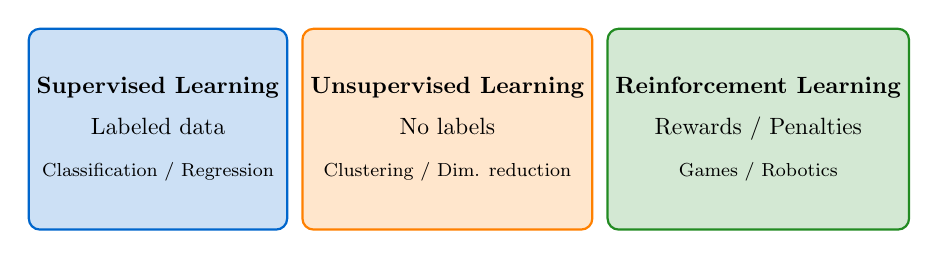
\begin{tikzpicture}[scale=0.85, every node/.style={transform shape}, node distance=0.2cm] % <-- increased spacing

% Box 1 - Supervised
\node[rectangle, draw=myblue, fill=myblue!20, thick, minimum width=3.5cm, minimum height=3cm, rounded corners, align=center] (sup) {
\textbf{Supervised Learning} \\[0.2cm]
Labeled data \\[0.2cm]
\footnotesize Classification / Regression
};

% Box 2 - Unsupervised
\node[rectangle, draw=myorange, fill=myorange!20, thick, minimum width=3.5cm, minimum height=3cm, rounded corners, align=center, right=of sup] (unsup) {
\textbf{Unsupervised Learning} \\[0.2cm]
No labels \\[0.2cm]
\footnotesize Clustering / Dim. reduction
};

% Box 3 - Reinforcement
\node[rectangle, draw=mygreen, fill=mygreen!20, thick, minimum width=3.5cm, minimum height=3cm, rounded corners, align=center, right=of unsup] (rl) {
\textbf{Reinforcement Learning} \\[0.2cm]
Rewards / Penalties \\[0.2cm]
\footnotesize Games / Robotics
};

\end{tikzpicture}
\end{center}

\vspace{0.5cm}

\begin{block}{Choosing the Type}
The type of learning depends on:
\begin{itemize}
    \item Whether labels are available
    \item The project's goal
    \item The nature of the problem
\end{itemize}
\end{block}
\end{frame}
\begin{frame}{Supervised Learning: Principle}
\vspace{-0.3cm}

  \begin{definition}
Learning from labeled examples to make predictions on new data
\end{definition}


\begin{center}
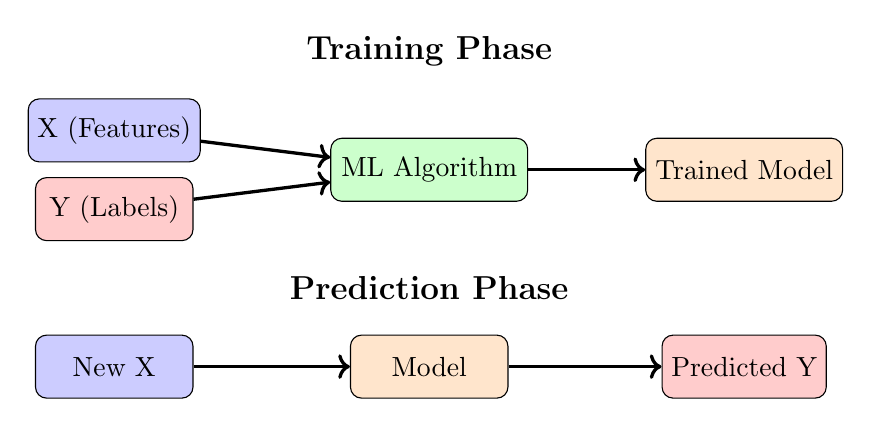
\begin{tikzpicture}

% Training Phase
\node[font=\large\bfseries] at (4,2.5) {Training Phase};

% Boxes
\node[draw, fill=blue!20, minimum width=2cm, minimum height=0.8cm, rounded corners] (x) at (0,1.5) {X (Features)};
\node[draw, fill=red!20, minimum width=2cm, minimum height=0.8cm, rounded corners] (y) at (0,0.5) {Y (Labels)};
\node[draw, fill=green!20, minimum width=2.5cm, minimum height=0.8cm, rounded corners] (algo) at (4,1) {ML Algorithm};
\node[draw, fill=orange!20, minimum width=2.5cm, minimum height=0.8cm, rounded corners] (modele) at (8,1) {Trained Model};

% Arrows
\draw[->, very thick] (x) -- (algo);
\draw[->, very thick] (y) -- (algo);
\draw[->, very thick] (algo) -- (modele);

% Prediction Phase
\node[font=\large\bfseries] at (4,-0.5) {Prediction Phase};

\node[draw, fill=blue!20, minimum width=2cm, minimum height=0.8cm, rounded corners] (xnew) at (0,-1.5) {New X};
\node[draw, fill=orange!20, minimum width=2cm, minimum height=0.8cm, rounded corners] (mod) at (4,-1.5) {Model};
\node[draw, fill=red!20, minimum width=2cm, minimum height=0.8cm, rounded corners] (ypred) at (8,-1.5) {Predicted Y};

\draw[->, very thick] (xnew) -- (mod);
\draw[->, very thick] (mod) -- (ypred);

\end{tikzpicture}
\end{center}

\end{frame}

\begin{frame}{Supervised Learning: Examples}
\begin{columns}[T]
\column{0.5\textwidth}
\textbf{Classification}
\begin{exampleblock}{Email Spam}
\begin{itemize}
\item \textbf{Input}: Email content
\item \textbf{Output}: Spam or Not
\item \textbf{Data}: 10,000 labeled emails
\end{itemize}
\end{exampleblock}

\begin{exampleblock}{Medical Diagnosis}
\begin{itemize}
\item \textbf{Input}: Symptoms, test results
\item \textbf{Output}: Sick or Healthy
\item \textbf{Data}: Medical records
\end{itemize}
\end{exampleblock}

\column{0.5\textwidth}
\textbf{Regression}
\begin{exampleblock}{Real Estate Prices}
\begin{itemize}
\item \textbf{Input}: Surface area, location
\item \textbf{Output}: Price in €
\item \textbf{Data}: Past sales
\end{itemize}
\end{exampleblock}

\begin{exampleblock}{Future Sales}
\begin{itemize}
\item \textbf{Input}: History, season
\item \textbf{Output}: Sales volume
\item \textbf{Data}: Historical data
\end{itemize}
\end{exampleblock}
\end{columns}
\end{frame}
\begin{frame}{Unsupervised Learning: Principle}
\begin{definition}
Discovering hidden structures in data without labels
\end{definition}

\vspace{0.5cm}

\begin{center}
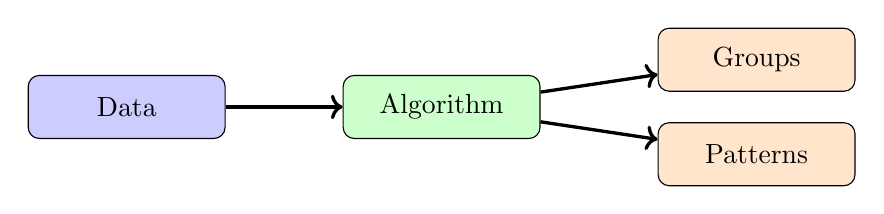
\begin{tikzpicture}

\node[draw, fill=blue!20, minimum width=2.5cm, minimum height=0.8cm, rounded corners] (data) at (0,0) {Data};
\node[draw, fill=green!20, minimum width=2.5cm, minimum height=0.8cm, rounded corners] (algo) at (4,0) {Algorithm};
\node[draw, fill=orange!20, minimum width=2.5cm, minimum height=0.8cm, rounded corners] (results) at (8,0.6) {Groups};
\node[draw, fill=orange!20, minimum width=2.5cm, minimum height=0.8cm, rounded corners] (patterns) at (8,-0.6) {Patterns};

\draw[->, very thick] (data) -- (algo);
\draw[->, very thick] (algo) -- (results);
\draw[->, very thick] (algo) -- (patterns);

\end{tikzpicture}
\end{center}

\vspace{0.3cm}
\begin{center}
\small The algorithm discovers the interesting structures on its own
\end{center}

\end{frame}

\begin{frame}{Unsupervised Learning: Examples}
\vspace{-25}
\begin{columns}[T]
\column{0.48\textwidth}
\begin{center}
\large\textbf{Clustering}
\end{center}

\begin{exampleblock}{Customer Segmentation}
\small
\begin{itemize}
\item \textbf{Input:} Age, income, purchases
\item \textbf{Output:} 4 customer groups
\item \textbf{Use:} Targeted marketing
\end{itemize}
\end{exampleblock}

\begin{exampleblock}{Document Organization}
\small
\begin{itemize}
\item \textbf{Input:} Article texts
\item \textbf{Output:} Similar topics
\item \textbf{Use:} Automatic classification
\end{itemize}
\end{exampleblock}

\column{0.48\textwidth}
\begin{center}
\large\textbf{Anomaly Detection}
\end{center}


\begin{exampleblock}{Bank Fraud}
\small
\begin{itemize}
\item \textbf{Input:} Transactions
\item \textbf{Output:} Suspicious transactions
\item \textbf{Use:} Security
\end{itemize}
\end{exampleblock}

\begin{exampleblock}{Predictive Maintenance}
\small
\begin{itemize}
\item \textbf{Input:} Sensor data
\item \textbf{Output:} Abnormal behavior
\item \textbf{Use:} Preventing failures
\end{itemize}
\end{exampleblock}

\end{columns}
\end{frame}

% ============================================
% SECTION 4: KEY CONCEPTS
% ============================================
\section{Key ML Concepts}

\begin{frame}{Overfitting vs Underfitting (1/2)}
\begin{block}{The Central Challenge of ML}
Finding the right balance between simplicity and complexity of the model
\end{block}

\vspace{0.3cm}

\begin{center}
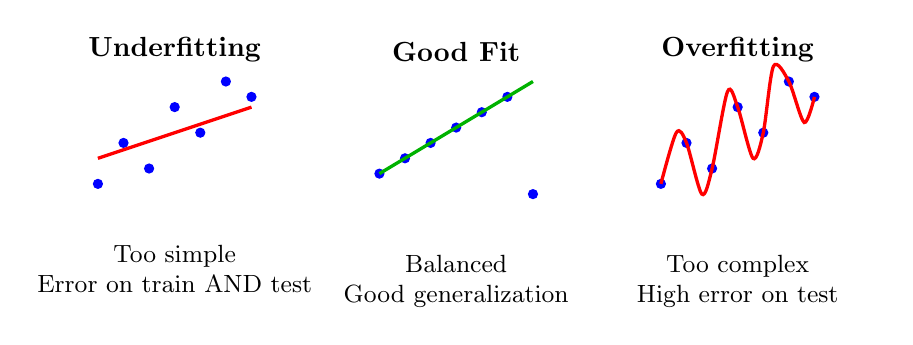
\begin{tikzpicture}[scale=0.65]

% Underfitting
\begin{scope}[shift={(0,0)}]
\node[above, font=\bfseries] at (2,3.2) {Underfitting};
% Data points
\foreach \x/\y in {0.5/1, 1/1.8, 1.5/1.3, 2/2.5, 2.5/2, 3/3, 3.5/2.7} {
    \fill[blue] (\x,\y) circle (0.1);
}
% Simple line
\draw[red, very thick] (0.5,1.5) -- (3.5,2.5);
\node[below, text width=3.5cm, align=center, font=\small] at (2,0) {Too simple\\Error on train AND test};
\end{scope}

% Good fit
\begin{scope}[shift={(5.5,0)}]
\node[above, font=\bfseries] at (2,3.2) {Good Fit};
% Points ON the line except ONE outlier
\foreach \x/\y in {0.5/1.2, 1/1.5, 1.5/1.8, 2/2.1, 2.5/2.4, 3/2.7, 3.5/0.8} {
    \fill[blue] (\x,\y) circle (0.1);
}
% Slightly less steep LINE
\draw[green!70!black, very thick] (0.5,1.2) -- (3.5,3);
\node[below, text width=3.5cm, align=center, font=\small] at (2,-0.2) {Balanced\\Good generalization};
\end{scope}

% Overfitting
\begin{scope}[shift={(11,0)}]
\node[above, font=\bfseries] at (2,3.2) {Overfitting};
% Points
\foreach \x/\y in {0.5/1, 1/1.8, 1.5/1.3, 2/2.5, 2.5/2, 3/3, 3.5/2.7} {
    \fill[blue] (\x,\y) circle (0.1);
}
% Complex curve
\draw[red, very thick, smooth] plot coordinates {(0.5,1) (0.8,2) (1,1.8) (1.3,0.8) (1.5,1.3) (1.8,2.8) (2,2.5) (2.3,1.5) (2.5,2) (2.7,3.3) (3,3) (3.3,2.2) (3.5,2.7)};
\node[below, text width=3.5cm, align=center, font=\small] at (2,-0.2) {Too complex\\High error on test};
\end{scope}

\end{tikzpicture}
\end{center}

\end{frame}

\begin{frame}{Overfitting vs Underfitting (2/2)}
\begin{columns}[T]
\column{0.5\textwidth}
\textbf{Underfitting}
\begin{itemize}
\item Model too simple
\item Doesn't capture the patterns
\item Poor performance everywhere
\end{itemize}

\textbf{Solutions:}
\begin{itemize}
\item More complex model
\item More features
\item Longer training
\end{itemize}

\column{0.5\textwidth}
\textbf{Overfitting}
\begin{itemize}
\item Model too complex
\item Memorizes the data
\item Good on train, poor on test
\end{itemize}

\textbf{Solutions:}
\begin{itemize}
\item More data
\item Regularization
\item Simpler model
\item Cross-validation
\end{itemize}
\end{columns}


\begin{alertblock}{Goal}
Build a model that \textbf{generalizes} well to new data
\end{alertblock}
\end{frame}

\begin{frame}{Bias and Variance: Definitions}
\vspace{-0.3cm}

\begin{block}{Bias}
\textbf{Error due to the simplicity of the model}
\begin{itemize}
\item The model makes overly simplistic assumptions
\item Doesn't capture the true relationship in the data
\item \textbf{High bias} $\rightarrow$ Underfitting
\item \textbf{Example:} Using a straight line for non-linear data
\end{itemize}
\end{block}
\vspace{-0.2cm}


\begin{block}{Variance}
\textbf{Sensitivity of the model to variations in the data}
\begin{itemize}
\item The model learns the noise in addition to the signal
\item Very sensitive to the training data
\item \textbf{High variance} $\rightarrow$ Overfitting
\item \textbf{Example:} Degree-20 polynomial for 10 points
\end{itemize}
\end{block}

\end{frame}

\begin{frame}{Bias-Variance Trade-off 1/2}
\vspace{-0.3cm}

\begin{center}
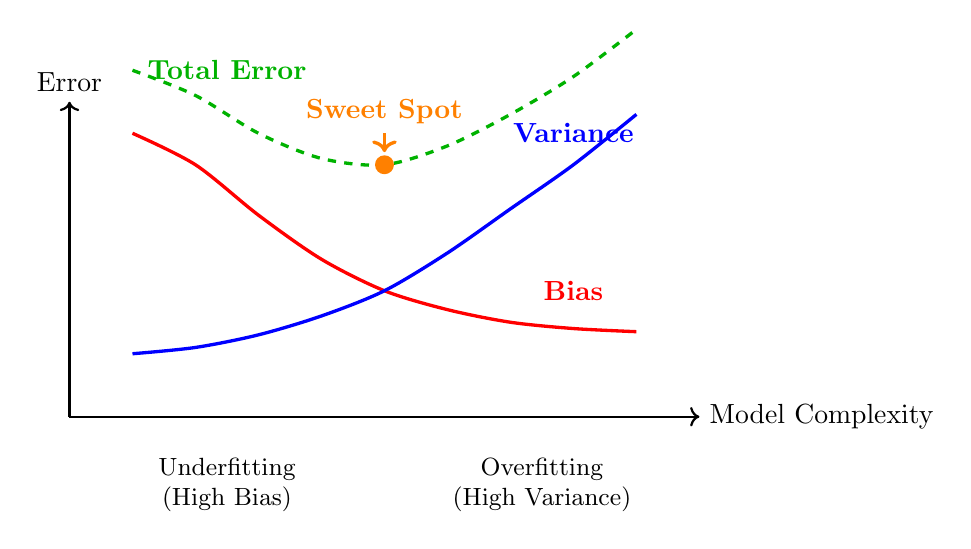
\begin{tikzpicture}[scale=0.8]
% Axes
\draw[->, thick] (0,0) -- (10,0) node[right] {Model Complexity};
\draw[->, thick] (0,0) -- (0,5) node[above] {Error};

% Bias curve
\draw[red, very thick, smooth] plot coordinates {(1,4.5) (2,4) (3,3.2) (4,2.5) (5,2) (6,1.7) (7,1.5) (8,1.4) (9,1.35)};
\node[red] at (8,2) {\textbf{Bias}};

% Variance curve
\draw[blue, very thick, smooth] plot coordinates {(1,1) (2,1.1) (3,1.3) (4,1.6) (5,2) (6,2.6) (7,3.3) (8,4) (9,4.8)};
\node[blue] at (8,4.5) {\textbf{Variance}};

% Total error
\draw[green!70!black, very thick, dashed, smooth] plot coordinates {(1,5.5) (2,5.1) (3,4.5) (4,4.1) (5,4) (6,4.3) (7,4.8) (8,5.4) (9,6.15)};
\node[green!70!black] at (2.5,5.5) {\textbf{Total Error}};

% Optimal point
\fill[orange] (5,4) circle (0.15);
\draw[->, orange, very thick] (5,4.5) -- (5,4.2);
\node[orange, above] at (5,4.5) {\textbf{Sweet Spot}};

% Zones
\node[below, text width=3cm, align=center, font=\small] at (2.5,-0.5) {Underfitting\\(High Bias)};
\node[below, text width=3cm, align=center, font=\small] at (7.5,-0.5) {Overfitting\\(High Variance)};

\end{tikzpicture}
\end{center}
\vspace{-0.4cm}
\end{frame}
\begin{frame}{Bias-Variance Trade-off 2/2} 
\begin{block}{The Trade-off}
\begin{itemize}
\item Reducing bias $\rightarrow$ increases variance
\item Reducing variance $\rightarrow$ increases bias
\item \textbf{Goal:} Find the optimal balance point
\end{itemize}
\end{block}
\end{frame}

\begin{frame}{Cross-Validation (1/2)}
\begin{block}{Problem}
How do we evaluate a model robustly when data is limited?
\end{block}

\begin{center}
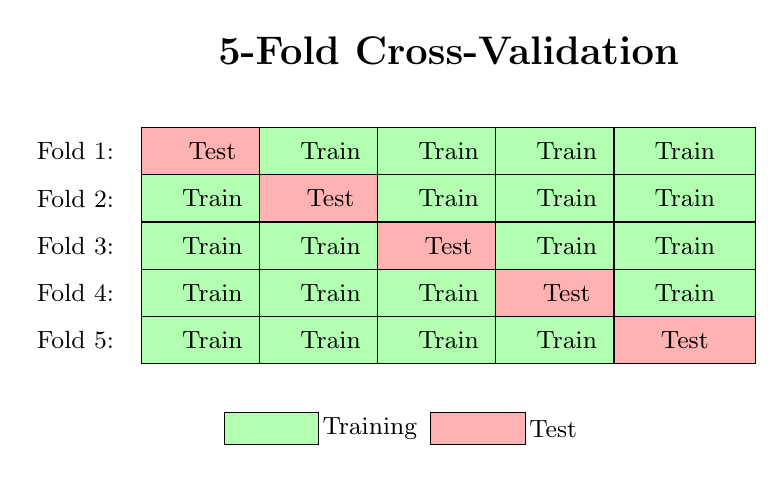
\begin{tikzpicture}[scale=0.75]
% K-Fold Cross Validation (K=5)
\node[above] at (5,4) {\Large \textbf{5-Fold Cross-Validation}};

\foreach \fold in {1,2,3,4,5} {
    % Compute vertical position
    \pgfmathsetmacro{\ypos}{3.5-0.8*\fold}
    
    % Fold name
    \node[left] at (-0.5,\ypos) {\small Fold \fold:};
    
    % The 5 blocks
    \foreach \block in {1,2,3,4,5} {
        \pgfmathsetmacro{\xpos}{\block*2-1}
        
        \ifnum\block=\fold
            % Test block (red)
            \node[rectangle, draw, fill=red!30, minimum width=1.8cm, minimum height=0.6cm] at (\xpos,\ypos) {\small Test};
        \else
            % Training block (green)
            \node[rectangle, draw, fill=green!30, minimum width=1.8cm, minimum height=0.6cm] at (\xpos,\ypos) {\small Train};
        \fi
    }
}

% Legend
\node[rectangle, draw, fill=green!30, minimum width=1.2cm, minimum height=0.4cm] at (2,-2) {};
\node[right] at (2.7,-2) {\small Training};
\node[rectangle, draw, fill=red!30, minimum width=1.2cm, minimum height=0.4cm] at (5.5,-2) {};
\node[right] at (6.2,-2) {\small Test};

\end{tikzpicture}
\end{center}
\end{frame}
\begin{frame}{Cross-Validation (2/2)}
\begin{block}{Advantage}
Every data point is used both for training and for testing → more reliable evaluation
\end{block}
\end{frame}

% ============================================
% SECTION 5: PRACTICAL EXAMPLES
% ============================================
\section{Practical Examples}

\begin{frame}{Example 1: Email Classification (Spam)}
\begin{columns}[T]
\column{0.5\textwidth}
\textbf{The Problem}
\begin{itemize}
\item Receiving thousands of emails
\item Automatically identifying spam
\item Avoiding false positives
\end{itemize}


\textbf{The Data}
\begin{itemize}
\item 10,000 labeled emails
\item Spam: 40\%
\item Non-spam (Ham): 60\%
\end{itemize}


\textbf{Possible Features}
\begin{itemize}
\item Specific words
\item Message length
\item Known/unknown sender
\end{itemize}

\column{0.5\textwidth}
\textbf{The Process}
\begin{enumerate}
\item Preparation
\begin{itemize}
\item Text cleaning
\item Feature extraction
\end{itemize}

\item Training
\begin{itemize}
\item Algorithm: SVM
\item Train: 8,000 emails
\end{itemize}

\item Test
\begin{itemize}
\item Test: 2,000 emails
\item Accuracy: 95\%
\end{itemize}

\item Deployment
\begin{itemize}
\item Automatic filter
\item Continuous improvement
\end{itemize}
\end{enumerate}
\end{columns}
\end{frame}

\begin{frame}{Example 2: Price Prediction (Real Estate)}
\begin{columns}[T]
\column{0.5\textwidth}
\textbf{The Problem}
\begin{itemize}
\item Estimating a house's price
\item Supporting buy/sell decisions
\item Regression problem
\end{itemize}


\textbf{The Data}
\begin{itemize}
\item 5,000 recent sales
\item Prices from €50k to €500k
\end{itemize}



\textbf{Features Used}
\begin{itemize}
\item Surface area (m²)
\item Number of bedrooms
\item Location (GPS)
\item Year built
\item Distance to city center
\end{itemize}

\column{0.5\textwidth}
\textbf{The Process}
\begin{enumerate}
\item Preparation
\begin{itemize}
\item Feature normalization
\item Location encoding
\end{itemize}

\item Training
\begin{itemize}
\item Algorithm: Linear Regression
\item Train: 4,000 houses
\end{itemize}

\item Test
\begin{itemize}
\item Test: 1,000 houses
\item Average error: ±€15k
\end{itemize}

\item Usage
\begin{itemize}
\item Input: house characteristics
\item Output: estimated price
\end{itemize}
\end{enumerate}
\end{columns}
\end{frame}

\begin{frame}{Example 3: Customer Segmentation (Clustering)}
\vspace{-0.3cm}

\begin{columns}[T]
\column{0.5\textwidth}
\textbf{The Problem}
\begin{itemize}
\item E-commerce with 50,000 customers
\item Need for homogeneous groups
\item Personalized marketing
\item Unsupervised learning
\end{itemize}


\textbf{The Data}
\begin{itemize}
\item Purchase history
\item Browsing behavior
\item Demographic data
\end{itemize}

\vspace{-0.2cm}

\textbf{Features}
\vspace{-0.1cm}

\begin{itemize}
\item Amount spent
\item Purchase frequency
\item Preferred categories
\item Age, location
\end{itemize}

\column{0.5\textwidth}
\textbf{The Process}
\vspace{-0.1cm}

\begin{enumerate}
\item Preparation
\vspace{-0.1cm}

\begin{itemize}
\item Normalization
\item Feature selection
\end{itemize}

\item Clustering
\begin{itemize}
\item Algorithm: K-Means
\item Choice K=4 groups
\end{itemize}

\item Results
\begin{itemize}
\item Group 1: VIP (5\%)
\item Group 2: Regulars (35\%)
\item Group 3: Occasional (45\%)
\item Group 4: Inactive (15\%)
\end{itemize}
\vspace{-0.2cm}
\item Action
\begin{itemize}
\item Personalized offers
\item Targeted campaigns
\end{itemize}
\end{enumerate}
\end{columns}
\end{frame}

% ============================================
% SECTION 6: TOOLS AND ECOSYSTEM
% ============================================
\section{ML Tools and Ecosystem}
\vspace{-0.3cm}

\begin{frame}{The Python Ecosystem for ML}
\vspace{-0.3cm}
\begin{columns}[T]
\column{0.48\textwidth}
\begin{center}
\vspace{-0.3cm}

\large\textbf{Essential Libraries}
\end{center}

\vspace{-0.3cm}

\begin{block}{NumPy}
\small Numerical computation and multidimensional arrays
\end{block}
\vspace{-0.2cm}

\begin{block}{Pandas}
\small Manipulation and analysis of tabular data
\end{block}

\begin{block}{Matplotlib / Seaborn}
\small Data visualization and plotting
\end{block}
\vspace{-0.2cm}

\begin{block}{Scikit-learn}
\small Classical ML algorithms and preprocessing
\end{block}
\vspace{-0.2cm}

\column{0.48\textwidth}
\begin{center}
\vspace{-0.3cm}

\large\textbf{Deep Learning Frameworks}
\end{center}
\vspace{-0.6cm}


\begin{block}{TensorFlow}
\small Google's framework for production
\end{block}
\vspace{-0.3cm}

\begin{block}{PyTorch}
\small Meta's framework for research
\end{block}
\vspace{-0.2cm}

\begin{block}{Keras}
\small High-level API for simplicity
\end{block}
\vspace{-0.3cm}


\begin{center}
\textbf{Development Environments}
\vspace{-0.6cm}

\end{center}
\small
\begin{itemize}
\item Jupyter Notebook
\vspace{-0.2cm}

\item Google Colab
\vspace{-0.2cm}

\item VS Code / PyCharm
\end{itemize}

\end{columns}
\end{frame}
\begin{frame}{Typical Workflow with Python}
\begin{center}
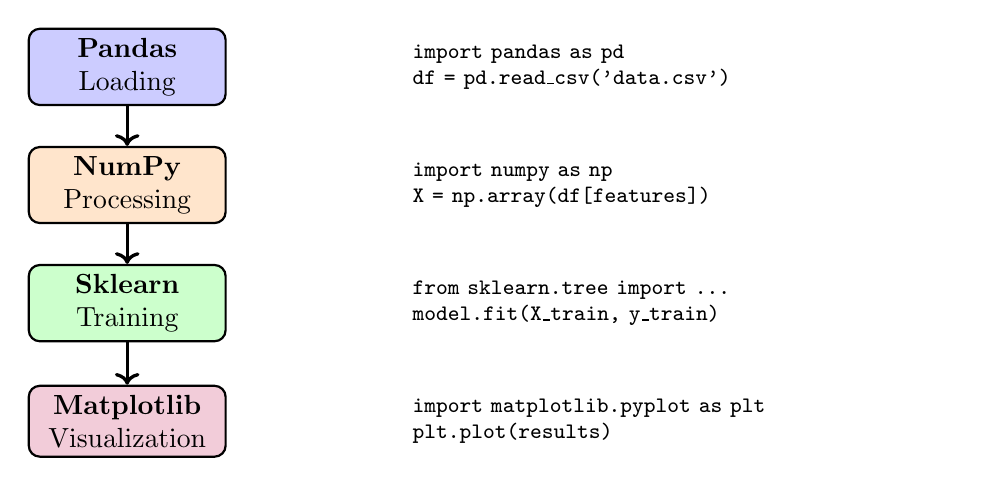
\begin{tikzpicture}[
box/.style={rectangle, draw, thick, rounded corners, minimum width=2.5cm, minimum height=0.8cm, align=center},
]

% Steps
\node[box, fill=blue!20] (pandas) at (0,3) {\textbf{Pandas}\\Loading};
\node[box, fill=orange!20] (numpy) at (0,1.5) {\textbf{NumPy}\\Processing};
\node[box, fill=green!20] (sklearn) at (0,0) {\textbf{Sklearn}\\Training};
\node[box, fill=purple!20] (viz) at (0,-1.5) {\textbf{Matplotlib}\\Visualization};

% Arrows
\draw[->, very thick] (pandas) -- (numpy);
\draw[->, very thick] (numpy) -- (sklearn);
\draw[->, very thick] (sklearn) -- (viz);

% Code examples on the right
\node[right, text width=7cm, font=\footnotesize\ttfamily] at (3.5,3) {
import pandas as pd\\
df = pd.read\_csv('data.csv')
};

\node[right, text width=7cm, font=\footnotesize\ttfamily] at (3.5,1.5) {
import numpy as np\\
X = np.array(df[features])
};

\node[right, text width=7cm, font=\footnotesize\ttfamily] at (3.5,0) {
from sklearn.tree import ...\\
model.fit(X\_train, y\_train)
};

\node[right, text width=7cm, font=\footnotesize\ttfamily] at (3.5,-1.5) {
import matplotlib.pyplot as plt\\
plt.plot(results)
};

\end{tikzpicture}
\end{center}
\end{frame}

% ============================================
% SECTION 7: BEST PRACTICES
% ============================================
\section{Best Practices and Advice}

\begin{frame}{The 10 Commandments of ML (1/2)}
\begin{enumerate}
\item \textbf{Start simple}
\begin{itemize}
\item Simple baseline before a complex model
\item Linear regression before deep learning
\end{itemize}

\item \textbf{Understand the data}
\begin{itemize}
\item Descriptive statistics
\item Exploratory visualization
\end{itemize}

\item \textbf{Rigorous cleaning}
\begin{itemize}
\item Check for missing values
\item Detect outliers
\end{itemize}

\item \textbf{Feature Engineering}
\begin{itemize}
\item Create relevant features
\item Test different transformations
\end{itemize}

\item \textbf{Proper validation}
\begin{itemize}
\item Train/Test split
\item Cross-validation
\end{itemize}
\end{enumerate}
\end{frame}

\begin{frame}{The 10 Commandments of ML (2/2)}
\begin{enumerate}
\setcounter{enumi}{5}
\item \textbf{Avoid overfitting}
\begin{itemize}
\item Regularization
\item More data
\end{itemize}

\item \textbf{Choose the right metrics}
\begin{itemize}
\item Based on the business problem
\item Not just accuracy
\end{itemize}

\item \textbf{Iterate and improve}
\begin{itemize}
\item Test several algorithms
\item Tune hyperparameters
\end{itemize}

\item \textbf{Document the work}
\begin{itemize}
\item Clear notebooks
\item Reproducibility
\end{itemize}

\item \textbf{Think about deployment}
\begin{itemize}
\item Production-ready code
\item Model monitoring
\end{itemize}
\end{enumerate}
\end{frame}

\begin{frame}{Common Pitfalls to Avoid}
\vspace{-0.3cm}
\begin{columns}[T]
\column{0.5\textwidth}
\textbf{Data Errors}
\begin{itemize}
\item Data leakage
\item Features from the future
\item Bias in the data
\item Class imbalance
\end{itemize}


\textbf{Modeling Errors}
\begin{itemize}
\item Overfitting
\item Underfitting
\item Poor validation
\item Ignoring outliers
\end{itemize}

\column{0.5\textwidth}
\textbf{Methodological Errors}
\begin{itemize}
\item Testing on training data
\item Optimizing on the test set
\item Ignoring business context
\item Features unavailable in production
\end{itemize}


\textbf{Communication Errors}
\begin{itemize}
\item Unrealistic promises
\item Ignoring limitations
\item No explanation of the model
\end{itemize}
\end{columns}


\begin{alertblock}{Important}
Most ML failures come from data problems, not algorithm problems!
\end{alertblock}
\end{frame}

% ============================================
% SECTION 8: CONCLUSION
% ============================================
\section{Conclusion}

\begin{frame}{What We Have Learned}
\begin{block}{Fundamental Concepts}
\begin{itemize}
\item Definition and principle of Machine Learning
\item Difference from classical programming
\item The complete ML pipeline
\item Types of learning (supervised, unsupervised)
\end{itemize}
\end{block}

\begin{block}{Key Concepts}
\begin{itemize}
\item Features and Labels
\item Train/Test split
\item Overfitting and Underfitting
\item Cross-validation
\item Bias-Variance trade-off
\end{itemize}
\end{block}

\begin{block}{Practice}
\begin{itemize}
\item Concrete examples (spam, prices, segmentation)
\item Python tools (Pandas, NumPy, Scikit-learn)
\item Best practices and pitfalls to avoid
\end{itemize}
\end{block}
\end{frame}

\begin{frame}{The ML Learning Path}

\begin{center}
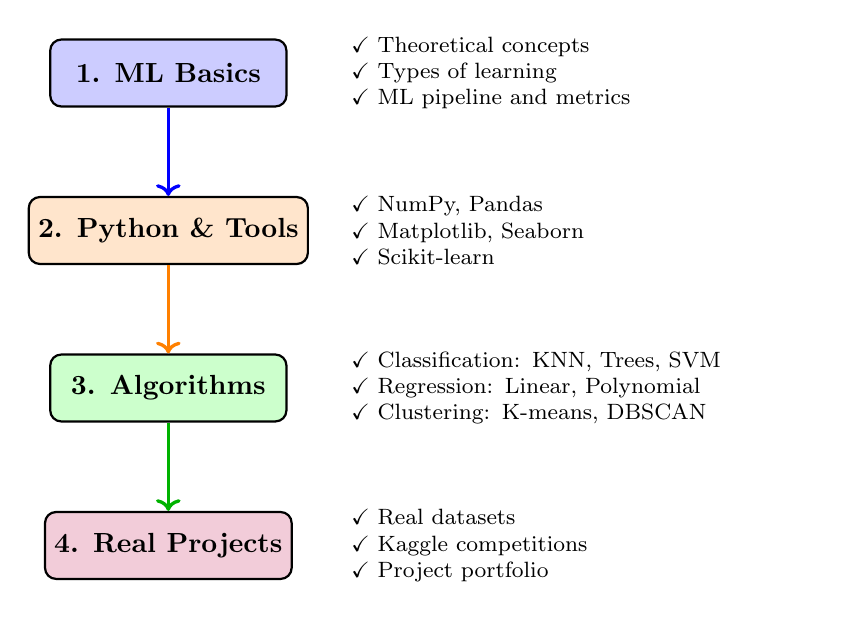
\begin{tikzpicture}

% Path stages
\node[rectangle, draw, thick, fill=blue!20, rounded corners, minimum width=3cm, minimum height=0.85cm] (bases) at (0,6) {\textbf{1. ML Basics}};
\node[rectangle, draw, thick, fill=orange!20, rounded corners, minimum width=3cm, minimum height=0.85cm] (python) at (0,4) {\textbf{2. Python \& Tools}};
\node[rectangle, draw, thick, fill=green!20, rounded corners, minimum width=3cm, minimum height=0.85cm] (algos) at (0,2) {\textbf{3. Algorithms}};
\node[rectangle, draw, thick, fill=purple!20, rounded corners, minimum width=3cm, minimum height=0.85cm] (projects) at (0,0) {\textbf{4. Real Projects}};

% Arrows
\draw[->, very thick, blue] (bases) -- (python);
\draw[->, very thick, orange] (python) -- (algos);
\draw[->, very thick, green!70!black] (algos) -- (projects);

% Details on the right - MORE SPACED OUT
\node[right, text width=6cm, align=left, font=\footnotesize] at (2.2,6) {
$\checkmark$ Theoretical concepts\\
$\checkmark$ Types of learning\\
$\checkmark$ ML pipeline and metrics
};

\node[right, text width=6cm, align=left, font=\footnotesize] at (2.2,4) {
$\checkmark$ NumPy, Pandas\\
$\checkmark$ Matplotlib, Seaborn\\
$\checkmark$ Scikit-learn
};

\node[right, text width=6cm, align=left, font=\footnotesize] at (2.2,2) {
$\checkmark$ Classification: KNN, Trees, SVM\\
$\checkmark$ Regression: Linear, Polynomial\\
$\checkmark$ Clustering: K-means, DBSCAN
};

\node[right, text width=6cm, align=left, font=\footnotesize] at (2.2,0) {
$\checkmark$ Real datasets\\
$\checkmark$ Kaggle competitions\\
$\checkmark$ Project portfolio
};

\end{tikzpicture}
\end{center}



\end{frame}

\begin{frame}{Next Step: Python for ML}
\begin{block}{Next Class}
We will learn the essential Python tools for ML:
\begin{itemize}
\item NumPy: array manipulation
\item Pandas: data analysis
\item Matplotlib: visualization
\item Scikit-learn: first ML models
\end{itemize}
\end{block}

\vspace{0.5cm}


\begin{block}{Recommended Resources}
\begin{itemize}
\item Install Anaconda (Python + libraries)
\item Create a free Google Colab account
\item Explore Kaggle for datasets
\end{itemize}
\end{block}
\end{frame}



\end{document}
